\documentclass[12pt,a4paper]{article}

\usepackage[utf8]{inputenc}
\usepackage[T2A]{fontenc}
\usepackage[ukrainian]{babel}

\usepackage{geometry}
\geometry{left=2cm,right=2cm,top=2cm,bottom=2cm}

\usepackage{graphicx}
\usepackage{array,multirow}
\usepackage{booktabs}
\usepackage{caption}

\usepackage{subcaption}

\usepackage{tcolorbox}

\renewcommand{\thetable}{№\arabic{table}}
\captionsetup[table]{name=Таблиця}

\usepackage{amsmath}
\usepackage{pdflscape}
\usepackage{xcolor}

\usepackage{fvextra}
\usepackage{upquote}

\usepackage{hyperref}

\captionsetup[subfigure]{labelformat=simple,labelsep=space}

\usepackage{minted}

\usemintedstyle{vs}
\setminted{linenos, breaklines, frame=single, fontsize=\small}

\RecustomVerbatimCommand{\VerbatimInput}{VerbatimInput}{
    breaklines=true,
    breaksymbolleft={}
}

% Узагальнений стиль для коду
\newminted{java}{
  fontsize=\small,
  baselinestretch=1.05,
  breaklines,
  linenos,
  frame=lines,
  framesep=2mm
}

% Консоль/PowerShell як plain text
\newminted{text}{
  fontsize=\small,
  breaklines,
  frame=single,
  bgcolor=gray!5
}

\begin{document}

    \begin{titlepage}

        % Картинка шапки (по центру, з відступом від верху)
        \begin{center}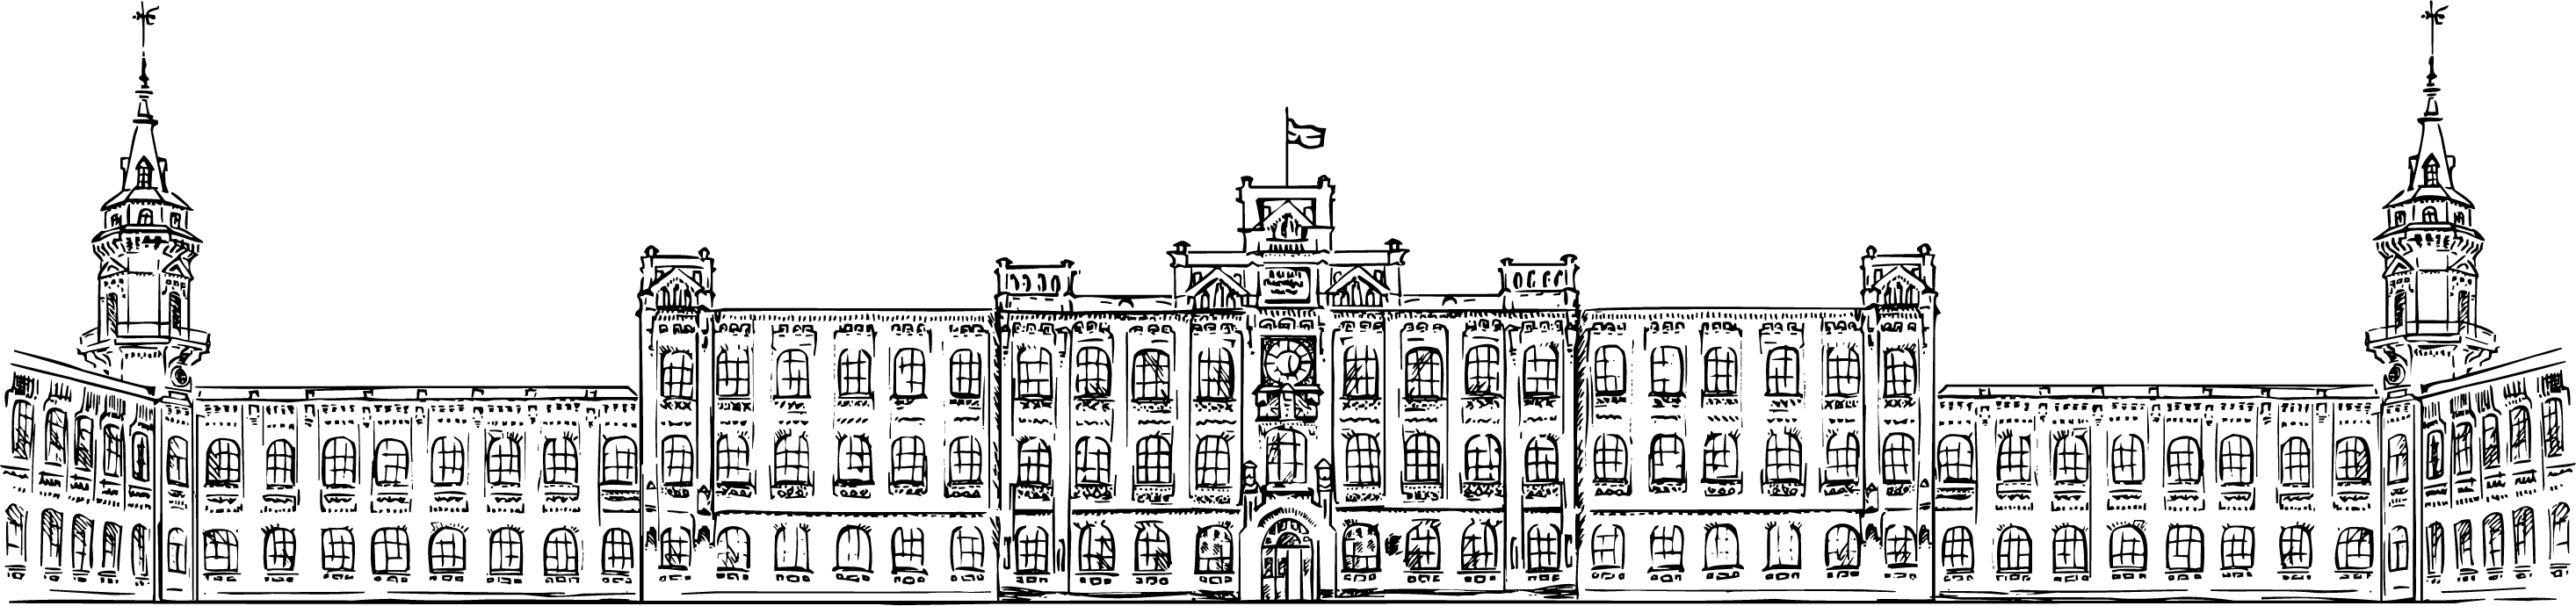
\includegraphics[width=0.7\textwidth]{../../../TITLES/letterhead.png}\end{center}

        \begin{center}
            \large Національний технічний університет України\\
            «Київський політехнічний інститут імені Ігоря Сікорського»\\[1em]
            Факультет інформатики та обчислювальної техніки\\
            Кафедра обчислювальної техніки
        \end{center}

        \vfill

        \begin{center}
            \textbf{\LARGE Інженерія програмного забезпечення}\\[2em]
            \textbf{\Large Практична робота №5}\\[0.5em]
            «Шаблони поведінки. Шаблони Visitor, Memento, State, Command, Interpreter»
        \end{center}

        \vfill

        \begin{flushright}
            Виконав: студент 2 курсу ФІОТ, гр. ІО-41\\
            \textit{Давидчук А.~М.}\\
            Залікова книжка № 4106\\[1em]
            Перевірив: \textit{Васильєва М.~Д.}
        \end{flushright}

        \vfill

        \begin{center}Київ --- 2025\end{center}

    \end{titlepage}

    % Основний документ:

    \setlength{\parindent}{0em}

    \textbf{\underline{Тема:}} «Шаблони поведінки. Шаблони Visitor, Memento, State, Command, Interpreter».

    \vspace{1em}

    \textbf{\underline{Мета:}} Ознайомлення з видами шаблонів проектування ПЗ. Вивчення шаблонів
    поведінки. Отримання базових навичок з застосування шаблонів Iterator, Mediator, Observer,
    Chain of Responsibility.

    \begin{center} \textbf{\Large Практична частина (Завдання №1)} \end{center}

    \setlength{\parindent}{1.5em}

    Мій номер залікової книги: $4106$, звідси $4106 \text{ mod } 8 = 2$. Тому умова до 1 завдання буде:

    Необхідно створити модель мережевої структури, що складається з таких типів елементів:
    \begin{itemize}
        \item \texttt{Cable} --- елемент, який представляє мережевий кабель;
        \item \texttt{Server} --- елемент, який представляє сервер;
        \item \texttt{Workstation} --- елемент, який представляє робочу станцію;
        \item \texttt{Network} --- комплексний елемент, який може містити інші елементи мережі (сервери, кабелі, робочі станції, а також вкладені підмережі).
    \end{itemize}

    Структура повинна підтримувати виконання додаткових операцій (наприклад, розрахунок вартості, відображення конфігурації тощо) \textbf{без внесення змін у класи елементів} (\texttt{Cable}, \texttt{Server}, \texttt{Workstation}, \texttt{Network}).

    \subsection*{Вимоги}

    \begin{itemize}
        \item \textbf{Абстрактний клас або інтерфейс елемента мережі (\texttt{NetworkElement}):}
        \begin{itemize}
            \item описує спільну поведінку всіх елементів мережі;
            \item повинен містити метод для прийому обробника (наприклад, \texttt{accept(Visitor v)}), який дозволяє елементу ``передати себе'' об'єкту, що виконує певну операцію.
        \end{itemize}

        \item \textbf{Реалізувати класи елементів мережі:}
        \begin{itemize}
            \item \texttt{Cable};
            \item \texttt{Server};
            \item \texttt{Workstation};
            \item \texttt{Network} (може містити інші елементи мережі, у тому числі вкладені об’єкти \texttt{Network}).
        \end{itemize}

        \item \textbf{Механізм розширення поведінки елементів мережі:}
        \begin{itemize}
            \item повинен дозволяти виконувати над елементами нові дії (розрахунок вартості, виведення структури, перевірка стану тощо) \textbf{без зміни коду класів елементів};
            \item для цього необхідно передбачити узгоджений набір методів обробки для кожного типу елемента.
        \end{itemize}

        \item \textbf{Клас, який реалізує конкретну операцію над елементами мережі:}
        \begin{itemize}
            \item наприклад, клас для розрахунку вартості мережі або для відображення її конфігурації;
            \item повинен містити окремі методи для обробки різних типів елементів: \texttt{Cable}, \texttt{Server}, \texttt{Workstation}, \texttt{Network}.
        \end{itemize}

        \item \textbf{Спеціальний метод прийому обробника в кожному елементі мережі:}
        \begin{itemize}
            \item елемент мережі не повинен знати, яку саме дію виконає обробник;
            \item елемент лише викликає метод обробника, передаючи йому себе як параметр (приклад: \texttt{visitor.visitCable(this);}).
        \end{itemize}
    \end{itemize}

    \subsection*{У методі \texttt{main} продемонструвати:}

    \begin{itemize}
        \item створення мережевої структури з декількох елементів (мережа, яка містить сервер, робочу станцію, кабелі, підмережі);
        \item виконання різних операцій над елементами мережі;
        \item можливість додавання нових типів операцій (наприклад, \texttt{Display} для відображення конфігурації або \texttt{CheckConnection} для перевірки зв'язності між вузлами) без зміни коду класів \texttt{Network}, \texttt{Server}, \texttt{Workstation}, \texttt{Cable}.
    \end{itemize}

    \setlength{\parindent}{0em}

    \textbf{\underline{Загальна структура проекту до компіляції:}}

    \begin{minted}{text}
PS C:\Users\artem\Desktop\reps\university_roadmap\semestr3\software engineering\labs\lab5\task1> tree /f /a
Folder PATH listing
Volume serial number is 1A5B-F8AF
C:.
|   build.xml
|   
\---src
    \---work5
            Cable.java
            CostCalculatorVisitor.java
            DisplayVisitor.java
            Network.java
            NetworkDemo.java
            NetworkElement.java
            NetworkVisitor.java
            Server.java
            Workstation.java
    \end{minted}

    \textbf{\underline{Код build.xml задля автоматизації:}}

    \begin{minted}{xml}
<?xml version="1.0" encoding="UTF-8"?>
<project name="task1" default="run" basedir=".">

    <!-- Основні директорії -->
    <property name="src.dir"   value="src"/>
    <property name="build.dir" value="build"/>
    <property name="dist.dir"  value="dist"/>
    <property name="doc.dir"   value="doc"/>

    <!-- Ініціалізація: створення службових папок -->
    <target name="init" description="Create build, dist and doc directories">
        <mkdir dir="${build.dir}"/>
        <mkdir dir="${dist.dir}"/>
        <mkdir dir="${doc.dir}"/>
    </target>

    <!-- Клас-пас для компіляції та запуску -->
    <path id="classpath">
        <pathelement path="${build.dir}"/>
    </path>

    <!-- Компіляція Java-джерел -->
    <target name="compile" depends="init" description="Compile Java sources">
        <javac srcdir="${src.dir}"
               destdir="${build.dir}"
               includeantruntime="false"
               source="1.8"
               target="1.8"
               debug="true"
               encoding="UTF-8">
            <classpath refid="classpath"/>
        </javac>
    </target>

    <!-- Створити виконуваний JAR-файл -->
    <target name="jar" depends="compile" description="Create runnable JAR archive">
        <jar destfile="${dist.dir}/task1.jar" basedir="${build.dir}">
            <manifest>
                <attribute name="Main-Class" value="work5.NetworkDemo"/>
            </manifest>
        </jar>
    </target>

    <!-- Запуск програми -->
    <target name="run" depends="compile,javadoc" description="Run demo program">
        <java classname="work5.NetworkDemo" fork="true">
            <classpath>
                <pathelement path="${build.dir}"/>
            </classpath>
        </java>
    </target>

    <!-- Генерація Javadoc-документації для пакету work5 -->
    <target name="javadoc" depends="compile" description="Generate Javadoc documentation">
        <javadoc destdir="${doc.dir}"
                 sourcepath="${src.dir}"
                 packagenames="work5"
                 encoding="UTF-8"
                 docencoding="UTF-8"
                 charset="UTF-8"
                 author="true"
                 version="true"
                 use="true"
                 windowtitle="task1 API"
                 doctitle="task1 API">
        </javadoc>
    </target>

    <!-- Прибирання результатів збірки -->
    <target name="clean" description="Delete build, dist and doc directories">
        <delete dir="${build.dir}"/>
        <delete dir="${dist.dir}"/>
        <delete dir="${doc.dir}"/>
    </target>

</project>
    \end{minted}

    \textbf{\underline{Перевірка:}}

    \begin{minted}{text}
PS C:\Users\artem\Desktop\reps\university_roadmap\semestr3\software engineering\labs\lab5\task1> ant -p 
Buildfile: C:\Users\artem\Desktop\reps\university_roadmap\semestr3\software engineering\labs\lab5\task1\build.xml

Main targets:

clean    Delete build, dist and doc directories
compile  Compile Java sources
init     Create build, dist and doc directories
jar      Create runnable JAR archive
javadoc  Generate Javadoc documentation
run      Run demo program
Default target: run
    \end{minted}

    Вихідний код буде на віддаленому репозиторії, посилання на яке буде додане разом із звітом.

    \textbf{\underline{Загальна структура проекту після виконання збірки:}}

    \begin{minted}{text}
PS C:\Users\artem\Desktop\reps\university_roadmap\semestr3\software engineering\labs\lab5\task1> tree /f /a
Folder PATH listing
Volume serial number is 1A5B-F8AF
C:.
|   build.xml
|   
+---build
|   \---work5
|           Cable.class
|           CostCalculatorVisitor.class
|           DisplayVisitor.class
|           Network.class
|           NetworkDemo.class
|           NetworkElement.class
|           NetworkVisitor.class
|           Server.class
|           Workstation.class
|
+---dist
+---doc
|   |   allclasses-index.html
|   |   allpackages-index.html
|   |   copy.svg
|   |   element-list
|   |   help-doc.html
|   |   index-all.html
|   |   index.html
|   |   link.svg
|   |   member-search-index.js
|   |   module-search-index.js
|   |   overview-tree.html
|   |   package-search-index.js
|   |   script.js
|   |   search-page.js
|   |   search.html
|   |   search.js
|   |   stylesheet.css
|   |   tag-search-index.js
|   |   type-search-index.js
|   |
|   +---legal
|   |       COPYRIGHT
|   |       jquery.md
|   |       jqueryUI.md
|   |       LICENSE
|   |
|   +---resources
|   |       glass.png
|   |       x.png
|   |
|   +---script-dir
|   |       jquery-3.7.1.min.js
|   |       jquery-ui.min.css
|   |       jquery-ui.min.js
|   |
|   \---work5
|       |   Cable.html
|       |   CostCalculatorVisitor.html
|       |   DisplayVisitor.html
|       |   Network.html
|       |   NetworkDemo.html
|       |   NetworkElement.html
|       |   NetworkVisitor.html
|       |   package-summary.html
|       |   package-tree.html
|       |   package-use.html
|       |   Server.html
|       |   Workstation.html
|       |
|       \---class-use
|               Cable.html
|               CostCalculatorVisitor.html
|               DisplayVisitor.html
|               Network.html
|               NetworkDemo.html
|               NetworkElement.html
|               NetworkVisitor.html
|               Server.html
|               Workstation.html
|
\---src
    \---work5
            Cable.java
            CostCalculatorVisitor.java
            DisplayVisitor.java
            Network.java
            NetworkDemo.java
            NetworkElement.java
            NetworkVisitor.java
            Server.java
            Workstation.java
    \end{minted}

    \textbf{\underline{Скріншот наявності документації:}}

    \begin{figure}[h!]
        \centering
        
\includegraphics[width=\linewidth]{1_1.png}
        \caption{Скріншот документації Javadoc для 1 завдання}
    \end{figure}

    \newpage

    \textbf{\underline{UML-діаграма проекту:}}

    \begin{figure}[h!]
        \centering
        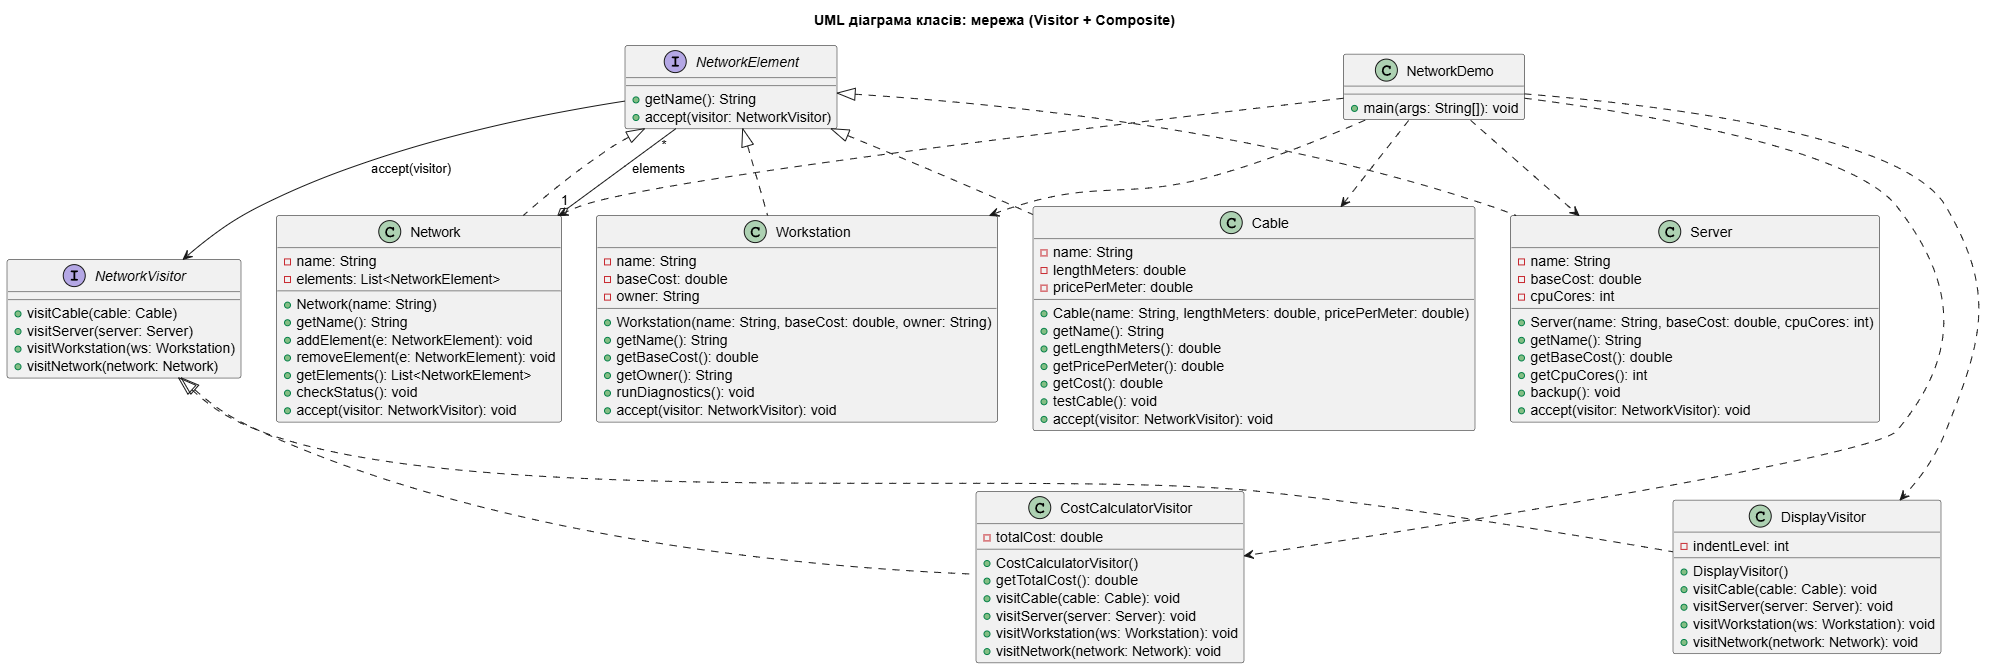
\includegraphics[width=\linewidth]{uml1.png}
        \caption{UML-діаграма проекту для 1 завдання}
    \end{figure}

    \setlength{\parindent}{1.5em}

    У пакеті \texttt{work5} реалізовано модель мережі згідно з варіантом:
    класи \texttt{Cable}, \texttt{Server}, \texttt{Workstation} і \texttt{Network}
    імплементують інтерфейс \texttt{NetworkElement}.
    
    Клас \texttt{Network} містить
    колекцію \texttt{List<NetworkElement>}, тобто мережа може включати сервери,
    робочі станції, кабелі та підмережі, що відповідає структурі шаблону
    \textit{Composite}. Для розширення поведінки без зміни цих класів використано
    шаблон \textit{Visitor}: інтерфейс \texttt{NetworkVisitor} та конкретні
    відвідувачі \texttt{DisplayVisitor} (виведення структури) і
    \texttt{CostCalculatorVisitor} (розрахунок загальної вартості). Нові операції
    можна додавати створенням нових відвідувачів без модифікації кодів елементів,
    як вимагає умова. У класах визначені бізнес-методи-заглушки
    (наприклад, \texttt{backup()}, \texttt{runDiagnostics()}), які лише виводять
    інформаційні повідомлення. Клас \texttt{NetworkDemo} у методі
    \texttt{main()} створює приклад мережі, викликає ці методи та демонструє роботу
    відвідувачів. Збірка, запуск та генерація Javadoc виконуються за допомогою
    \texttt{Ant} через файл \texttt{build.xml}, що підтверджується успішним
    \texttt{BUILD SUCCESSFUL}.

    \begin{center} \textbf{\Large Практична частина (Завдання №2)} \end{center}

    Мій номер залікової книги: $4106$, звідси $4106 \text{ mod } 7 = 4$. Тому умова до 2 завдання буде:

    Необхідно створити модель взаємодії користувача з пунктами меню та кнопками інструментальної панелі, яка включає такі елементи:
    \begin{itemize}
        \item \texttt{Action} (\textbf{Дія}) --- абстрактний опис реакції на натискання
        кнопки або вибір пункту меню;
        \item \texttt{ConcreteAction} (\textbf{Конкретна дія}) --- конкретні реалізації дій,
        які визначають, що відбувається при натисканні (наприклад,
        \texttt{SaveFileAction}, \texttt{OpenFileAction}, \texttt{CopyAction},
        \texttt{PasteAction});
        \item \texttt{Invoker} (\textbf{Ініціатор}) --- клас, який відповідає за
        ``натискання'' кнопок чи вибір пунктів меню і передачу виконання дій
        відповідним об’єктам \texttt{Action}.
    \end{itemize}

    \subsection*{Вимоги}

    \begin{itemize}
        \item Створити інтерфейс або абстрактний клас \texttt{Action}, який описує метод
        \texttt{execute()}.
        \item Реалізувати декілька класів дій
        (\texttt{SaveFileAction}, \texttt{OpenFileAction}, \texttt{CopyAction},
        \texttt{PasteAction}), які наслідують \texttt{Action}. Кожен клас визначає,
        яка поведінка відбувається при взаємодії користувача.
        \item Клас \texttt{Invoker} має містити посилання на поточну дію. Натискання
        кнопки чи вибір пункту меню викликає метод \texttt{execute()} поточної дії.
        Зміна дії динамічно змінює реакцію \texttt{Invoker} без використання
        умовних операторів.
        \item Реалізувати можливість формування макро-реакцій --- послідовностей дій,
        що виконуються за одного виклику (клас \texttt{MacroAction}, який містить список
        об’єктів \texttt{Action} і при виконанні викликає \texttt{execute()} для кожної
        з них).
    \end{itemize}

    \subsection*{У методі \texttt{main} продемонструвати}

    \begin{itemize}
        \item створення кількох дій (\texttt{Save}, \texttt{Open}, \texttt{Copy},
        \texttt{Paste}) та об’єкта \texttt{Invoker};
        \item виконання натискань кнопок і демонстрацію того, що \texttt{Invoker}
        делегує поведінку поточній дії;
        \item динамічну зміну дії \texttt{Invoker} та демонстрацію нової поведінки
        без використання умовних операторів.
    \end{itemize}

    \textbf{\underline{Загальна структура проекту до компіляції:}}

    \begin{minted}{text}
PS C:\Users\artem\Desktop\reps\university_roadmap\semestr3\software engineering\labs\lab5\task2> tree /f /a
Folder PATH listing
Volume serial number is 1A5B-F8AF
C:.
|   build.xml
|   
\---src
    \---work5
            Action.java
            ActionDemo.java
            CopyAction.java
            Invoker.java
            MacroAction.java
            OpenFileAction.java
            PasteAction.java
            SaveFileAction.java
    \end{minted}

    \textbf{\underline{Код build.xml задля автоматизації:}}

    \begin{minted}{xml}
<?xml version="1.0" encoding="UTF-8"?>
<project name="task2" default="run" basedir=".">

    <!-- Основні директорії проєкту -->
    <property name="src.dir"   value="src"/>
    <property name="build.dir" value="build"/>
    <property name="dist.dir"  value="dist"/>
    <property name="doc.dir"   value="doc"/>

    <!-- Початкова ініціалізація: створення службових папок -->
    <target name="init" description="Create build, dist and doc directories">
        <mkdir dir="${build.dir}"/>
        <mkdir dir="${dist.dir}"/>
        <mkdir dir="${doc.dir}"/>
    </target>

    <!-- Клас-пас для компіляції та запуску -->
    <path id="classpath">
        <pathelement path="${build.dir}"/>
    </path>

    <!-- Компіляція вихідних Java-файлів -->
    <target name="compile" depends="init" description="Compile Java sources">
        <javac srcdir="${src.dir}"
               destdir="${build.dir}"
               includeantruntime="false"
               source="1.8"
               target="1.8"
               debug="true"
               encoding="UTF-8">
            <classpath refid="classpath"/>
        </javac>
    </target>

    <!-- Генерація Javadoc-документації для пакета work5 -->
    <target name="javadoc" depends="compile" description="Generate Javadoc documentation">
        <javadoc destdir="${doc.dir}"
                 sourcepath="${src.dir}"
                 packagenames="work5"
                 encoding="UTF-8"
                 docencoding="UTF-8"
                 charset="UTF-8"
                 author="true"
                 version="true"
                 use="true"
                 windowtitle="task2 API"
                 doctitle="task2 API">
        </javadoc>
    </target>

    <!-- Створення виконуваного JAR-архіву -->
    <target name="jar" depends="compile" description="Create runnable JAR archive">
        <jar destfile="${dist.dir}/task2.jar" basedir="${build.dir}">
            <manifest>
                <attribute name="Main-Class" value="work5.ActionDemo"/>
            </manifest>
        </jar>
    </target>

    <!-- Запуск демо-програми -->
    <target name="run" depends="compile,javadoc" description="Run demo program">
        <java classname="work5.ActionDemo" fork="true">
            <classpath>
                <pathelement path="${build.dir}"/>
            </classpath>
        </java>
    </target>

    <!-- Очищення результатів збірки -->
    <target name="clean" description="Delete build, dist and doc directories">
        <delete dir="${build.dir}"/>
        <delete dir="${dist.dir}"/>
        <delete dir="${doc.dir}"/>
    </target>

</project>
    \end{minted}

    \textbf{\underline{Перевірка:}}

    \begin{minted}{text}
PS C:\Users\artem\Desktop\reps\university_roadmap\semestr3\software engineering\labs\lab5\task2> ant -p 
Buildfile: C:\Users\artem\Desktop\reps\university_roadmap\semestr3\software engineering\labs\lab5\task2\build.xml

Main targets:

 clean    Delete build, dist and doc directories
 compile  Compile Java sources
 init     Create build, dist and doc directories
 jar      Create runnable JAR archive
 javadoc  Generate Javadoc documentation
 run      Run demo program
Default target: run
    \end{minted}

    Вихідний код буде на віддаленому репозиторії, посилання на яке буде додане разом із звітом.

    \textbf{\underline{Загальна структура проекту після виконання збірки:}}

    \begin{minted}{text}
PS C:\Users\artem\Desktop\reps\university_roadmap\semestr3\software engineering\labs\lab5\task2> tree /f /a
Folder PATH listing
Volume serial number is 1A5B-F8AF
C:.
|   build.xml
|
+---build
|   \---work5
|           Action.class
|           ActionDemo.class
|           CopyAction.class
|           Invoker.class
|           MacroAction.class
|           OpenFileAction.class
|           PasteAction.class
|           SaveFileAction.class
|
+---dist
+---doc
|   |   allclasses-index.html
|   |   allpackages-index.html
|   |   copy.svg
|   |   element-list
|   |   help-doc.html
|   |   index-all.html
|   |   index.html
|   |   link.svg
|   |   member-search-index.js
|   |   module-search-index.js
|   |   overview-tree.html
|   |   package-search-index.js
|   |   script.js
|   |   search-page.js
|   |   search.html
|   |   search.js
|   |   stylesheet.css
|   |   tag-search-index.js
|   |   type-search-index.js
|   |
|   +---legal
|   |       COPYRIGHT
|   |       jquery.md
|   |       jqueryUI.md
|   |       LICENSE
|   |
|   +---resources
|   |       glass.png
|   |       x.png
|   |
|   +---script-dir
|   |       jquery-3.7.1.min.js
|   |       jquery-ui.min.css
|   |       jquery-ui.min.js
|   |
|   \---work5
|       |   Action.html
|       |   ActionDemo.html
|       |   CopyAction.html
|       |   Invoker.html
|       |   MacroAction.html
|       |   OpenFileAction.html
|       |   package-summary.html
|       |   package-tree.html
|       |   package-use.html
|       |   PasteAction.html
|       |   SaveFileAction.html
|       |
|       \---class-use
|               Action.html
|               ActionDemo.html
|               CopyAction.html
|               Invoker.html
|               MacroAction.html
|               OpenFileAction.html
|               PasteAction.html
|               SaveFileAction.html
|
\---src
    \---work5
            Action.java
            ActionDemo.java
            CopyAction.java
            Invoker.java
            MacroAction.java
            OpenFileAction.java
            PasteAction.java
            SaveFileAction.java
    \end{minted}

    \textbf{\underline{Скріншот наявності документації:}}

    \begin{figure}[h!]
        \centering
        
\includegraphics[width=\linewidth]{1_2.png}
        \caption{Скріншот документації Javadoc для 2 завдання}
    \end{figure}

    \newpage

    \textbf{\underline{UML-діаграма проекту:}}

    \begin{figure}[h!]
        \centering
        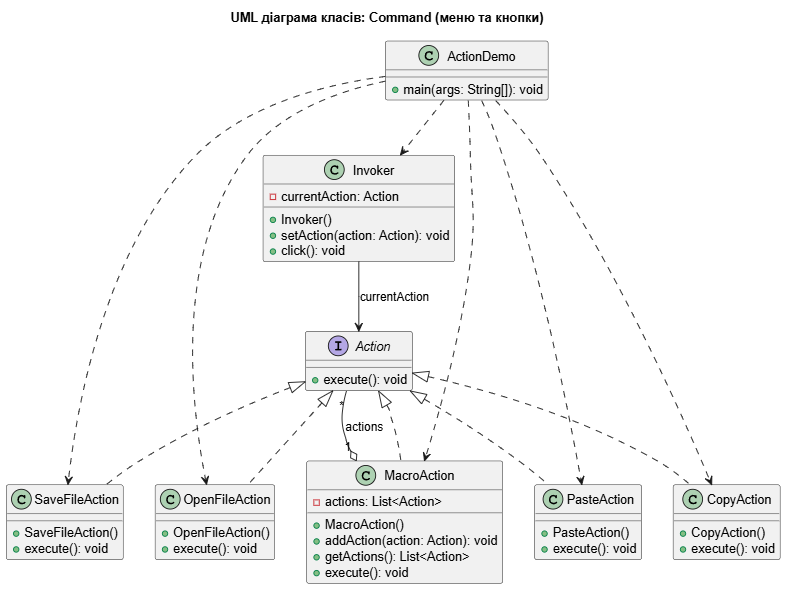
\includegraphics[width=\linewidth]{uml2.png}
        \caption{UML-діаграма проекту для 2 завдання}
    \end{figure}

    У пакеті \texttt{work5} реалізовано модель взаємодії користувача з пунктами меню
    та кнопками інструментальної панелі відповідно до варіанту. Базовий інтерфейс
    \texttt{Action} визначає єдиний метод \texttt{execute()}, який описує абстрактну
    дію. Конкретні класи \texttt{SaveFileAction}, \texttt{OpenFileAction},
    \texttt{CopyAction} та \texttt{PasteAction} реалізують інтерфейс \texttt{Action}
    і моделюють окремі команди (збереження, відкриття, копіювання, вставку).

    Клас \texttt{MacroAction} також реалізує \texttt{Action} і містить колекцію
    об'єктів \texttt{Action}; при виклику \texttt{execute()} він послідовно виконує
    усі вкладені дії, що відповідає вимозі формування макро-реакцій. Клас
    \texttt{Invoker} зберігає посилання на поточну дію \texttt{Action} та в методі
    \texttt{click()} просто викликає \texttt{execute()} цієї дії, тобто динамічна
    зміна поведінки досягається через \texttt{setAction()} без використання
    умовних операторів \texttt{if}/\texttt{switch}. У класі \texttt{ActionDemo} в
    методі \texttt{main()} створюються окремі дії, макро-дія та об'єкт
    \texttt{Invoker}, демонструється виконання одиночних команд і макро-команди, що
    підтверджує коректну реалізацію шаблону \textit{Command} та повну відповідність
    умовам завдання.

    \newpage

    \noindent
    \textbf{\underline{Висновок:}} У ході виконання лабораторної роботи було закріплено теоретичні знання щодо
шаблонів поведінки у проектуванні ПЗ та продемонстровано їх практичне
застосування на прикладах.

У першому завданні було реалізовано модель мережевої структури з використанням
шаблону \textit{Visitor} (та фактично \textit{Composite} для ієрархії елементів).
Інтерфейс \texttt{NetworkElement} і конкретні класи \texttt{Cable},
\texttt{Server}, \texttt{Workstation}, \texttt{Network} дозволили побудувати
деревоподібну структуру мережі, а відвідувачі \texttt{DisplayVisitor} та
\texttt{CostCalculatorVisitor} показали можливість додавання нових операцій над
елементами без зміни їхнього коду. Це відповідає принципам розширюваності та
слабкого зв’язку між структурами даних та операціями над ними.

У другому завданні було реалізовано шаблон \textit{Command} для моделювання
взаємодії користувача з меню та кнопками. Інтерфейс \texttt{Action} та
конкретні команди \texttt{SaveFileAction}, \texttt{OpenFileAction},
\texttt{CopyAction}, \texttt{PasteAction} інкапсулюють окремі дії, тоді як
клас \texttt{Invoker} делегує виконання поточній команді без використання
умовних конструкцій.

Клас \texttt{MacroAction} продемонстрував можливість
об’єднання кількох команд у єдину макро-операцію. Таким чином, було показано,
як шаблон \textit{Command} забезпечує гнучку зміну поведінки об’єкта під час
виконання програми.

Окрім цього, для обох завдань було налаштовано збірку проєктів за допомогою
системи \texttt{Ant} та автоматичну генерацію документації засобами
\texttt{Javadoc}, що сприяє підвищенню якості супроводу коду. У підсумку
лабораторна робота дозволила не лише засвоїти призначення та структуру
шаблонів \textit{Visitor} і \textit{Command}, але й отримати практичні навички
їх реалізації в мові Java в контексті реалістичних задач.

\end{document}